\documentclass{beamer}
%
% Choose how your presentation looks.
%
% For more themes, color themes and font themes, see:
% http://deic.uab.es/~iblanes/beamer_gallery/index_by_theme.html
%

\mode<presentation>
{
%  \usetheme{Berlin}      % or try Darmstadt, Madrid, Warsaw, ...
	\usetheme[
		bullet=circle,                  % Use circles instead of squares for bullets
		titleline=false,                % Show a line below the frame
		alternativetitlepage=true,      % Use the fancy title
		titlepagelogo=logo-sapienza,    % Logo for the first slide
		watermark=watermark-sapienza,   % Watermark used in every slide
		watermarkheight=20px,           % Desired height of the watermark
		watermarkheightmult=6,          % Watermark image is actually x times bigger
		displayauthoronfooter=true		
	]{Roma}
%  \usecolortheme{beaver} % or try albatross, beaver, crane, ...
%  \usefonttheme{default}  % or try serif, structurebold, ...
%  \setbeamertemplate{navigation symbols}{}
%  \setbeamertemplate{caption}[numbered]
} 



\usepackage[english]{babel}
\usepackage[utf8x]{inputenc}

%other packages...
\usepackage{hyperref}
\usepackage{xspace}
\usepackage{tabularx} % in the preamble
%\usepackage{subfigure}
\usepackage{subfig}
%\usepackage{chngcntr}
%\counterwithin{subfigure}{figure}
% The algorithm packages have to be after hyperref.
\usepackage{algorithm}
\usepackage{algpseudocode}
\usepackage{multirow}
\usepackage{animate}
\usepackage{tasks}

\usepackage{adjustbox}
\usepackage{multimedia}
%\usepackage{movie15}



\usepackage{tikz}
\usetikzlibrary{arrows}
% For every picture that defines or uses external nodes, you'll have to
% apply the 'remember picture' style. To avoid some typing, we'll apply
% the style to all pictures.
\tikzstyle{every picture}+=[remember picture]

% By default all math in TikZ nodes are set in inline mode. Change this to
% displaystyle so that we don't get small fractions.
\everymath{\displaystyle}
\tikzstyle{na} = [baseline=-.5ex]


%%%%%%%%%%%%%%%%%%%%%%%%%% General
\newcommand{\Section}[1]{Section \ref{#1}}

\newcommand{\myi}{(\emph{i})\xspace}
\newcommand{\myii}{(\emph{ii})\xspace}
\newcommand{\myiii}{(\emph{iii})\xspace}
\newcommand{\myiv}{(\emph{iv})\xspace}
\newcommand{\myv}{(\emph{v})\xspace}
\newcommand{\myvi}{(\emph{vi})\xspace}
\newcommand{\myvii}{(\emph{vii})\xspace}
\newcommand{\myviii}{(\emph{viii})\xspace}

%% general math
%\newcommand{\A}{\mathcal{A}} 
\newcommand{\B}{\mathcal{B}}
%\newcommand{\C}{\mathcal{C}} 
\newcommand{\D}{\mathcal{D}}
\newcommand{\E}{\mathcal{E}} \newcommand{\F}{\mathcal{F}}
\newcommand{\G}{\mathcal{G}} \renewcommand{\H}{\mathcal{H}}
\newcommand{\I}{\mathcal{I}} \newcommand{\J}{\mathcal{J}}
\newcommand{\K}{\mathcal{K}} \renewcommand{\L}{\mathcal{L}}
\newcommand{\M}{\mathcal{M}} \newcommand{\N}{\mathcal{N}}
\renewcommand{\O}{\mathcal{O}} \renewcommand{\P}{\mathcal{P}}
\newcommand{\Q}{\mathcal{Q}} \newcommand{\R}{\mathcal{R}}
\renewcommand{\S}{\mathcal{S}} \newcommand{\T}{\mathcal{T}}
\newcommand{\U}{\mathcal{U}} \newcommand{\V}{\mathcal{V}}
\newcommand{\W}{\mathcal{W}} \newcommand{\X}{\mathcal{X}}
\newcommand{\Y}{\mathcal{Y}} \newcommand{\Z}{\mathcal{Z}}

\newcommand{\limp}{\mathbin{\rightarrow}}
\newcommand{\ind}{\hspace*{.18in}}

%% LTL
\newcommand{\Atom}{A}
\newcommand{\Next}{\raisebox{-0.27ex}{\LARGE$\circ$}}
\newcommand{\Wnext}{\raisebox{-0.27ex}{\LARGE$\bullet$}}
\newcommand{\lUntil}{\mathop{\U}}
\newcommand{\Since}{\mathop{\S}}
\newcommand{\Release}{\mathop{\R}}
\newcommand{\Wuntil}{\mathop{\W}}
\newcommand{\true}{\mathit{true}}
\newcommand{\final}{\mathit{Final}}
\newcommand{\false}{\mathit{false}}
\newcommand{\ttrue}{{\mathit{tt}}}
\newcommand{\ffalse}{\mathit{ff}}
\newcommand{\Last}{\mathit{Last}}
\newcommand{\Ended}{\mathit{End}}
\newcommand{\length}{\mathit{length}}
\newcommand{\last}{\mathit{last}}
\newcommand{\End}{\mathit{end}}
\newcommand{\nnf}{\mathit{nnf}}
\newcommand{\BOX}[1]{ [#1]}
\newcommand{\DIAM}[1]{\langle #1 \rangle}
\newcommand{\transl}{f}


%% Logics
\newcommand{\LT}{{\sc lt}$_f$\xspace}
\newcommand{\LTi}{{\sc lt}$_i$\xspace}
\newcommand{\PLTL}{{\sc pltl}\xspace}
\newcommand{\FLTL}{{\sc \$fltl}\xspace}
\newcommand{\FstarLTL}{{\sc \$$^*$fltl}\xspace}
\newcommand{\PL}{{\sc pl}\xspace}
\newcommand{\LTL}{{\sc ltl}\xspace}
\newcommand{\LTLf}{{\sc ltl}$_f$\xspace}
\newcommand{\LDL}{{\sc ldl}\xspace}
\newcommand{\LDLf}{{\sc ldl}$_f$\xspace}
\newcommand{\RE}{{\sc re}$_f$\xspace}
\newcommand{\REGEX}{{\sc re}\xspace}
\newcommand{\DL}{{\sc dl}\xspace}
\newcommand{\PDL}{{\sc pdl}\xspace}
\newcommand{\FOf}{{\sc fo}$_f$\xspace}
\newcommand{\MSOf}{{\sc mso}$_f$\xspace}
\newcommand{\FO}{{\sc fo}\xspace}
\newcommand{\FOL}{{\sc fol}\xspace}
\newcommand{\MSO}{{\sc mso}\xspace}
%\newcommand{\ATA}{{\sc ata}\xspace}
\newcommand{\AFW}{{\sc afw}\xspace}
\newcommand{\NFA}{{\sc nfa}\xspace}
\newcommand{\DFA}{{\sc dfa}\xspace}
\newcommand{\DFAs}{{\sc dfa}s\xspace}
\newcommand{\declare}{{\sc declare}\xspace}
\newcommand{\fol}{\mathit{fol}}
\newcommand{\f}{\mathit{f}}
%\newcommand{\g}{\mathit{g}}
\newcommand{\re}{\mathit{re}}


\newcommand{\tup}[1]{\langle #1 \rangle}

\newcommand{\Stop}{\mathit{stop}}
\newcommand{\rew}{\mathit{rew}}
\newcommand{\Tr}{\mathit{Tr}}

\newcommand{\LOGSPACE}{{\sc logspace}\xspace}
\newcommand{\NLOGSPACE}{{\sc nlogspace}\xspace}
\newcommand{\PTIME}{{\sc ptime}\xspace}
\newcommand{\NP}{{\sc np}\xspace}
\newcommand{\EXPTIME}{{\sc exptime}\xspace}
\newcommand{\PSPACE}{{\sc pspace}\xspace}
\newcommand{\TWOEXPTIME}{{\sc 2exptime}\xspace}


\newcommand{\expand}{\textbf{\textit{E}}}
\newcommand{\ttt}{{\textbf{\textit{T}}}}
\newcommand{\fff}{{\textbf{\textit{\texttt{F}}}}}

\newcommand{\fstate}{s_f}

\newcommand{\atomize}[1]{\texttt{"}\ensuremath{#1}\texttt{"}}


% misc


%RL
\newcommand{\MDP}{\M}
\newcommand{\States}{S}
\newcommand{\Actions}{A}
\newcommand{\TrFun}{T}
\newcommand{\Reward}{R}
\newcommand{\DiscFact}{\gamma}
\newcommand{\Policy}{\rho}
\newcommand{\ExpRet}{G}
\newcommand{\ValFun}{v}
\newcommand{\qFun}{q}

\newcommand{\ValOptFun}{\ValFun^*}
\newcommand{\qOptFun}{\qFun^*}
\newcommand{\OptPolicy}{\Policy^*}

\newcommand{\ValFunEst}{V}
\newcommand{\qFunEst}{Q}
\newcommand{\LRate}{\alpha}

\newcommand{\NMRDP}{\N}
\newcommand{\NMReward}{\bar{\Reward}}
\newcommand{\NMPolicy}{\bar{\Policy}}

\newcommand{\traj}{\tup{s_0, a_0, \dots, s_{n-1}, a_{n-1}, s_n}}
\newcommand{\trajprime}{\tup{s'_0, a_0, \dots, s'_{n-1}, a_{n-1}, s'_n}}
\newcommand{\projtraj}{\tup{s_0, s_1, \dots, s_n}}
\newcommand{\projtrajprime}{\tup{s'_0, s'_1, \dots, s'_n}}

\newcommand{\MDPagent}{\MDP_{ag}}
\newcommand{\TrFunAgentGoal}{\TrFun_{ag}^{g}}

\newcommand{\bqs}{\mathbf{q}}

%LOGIC

\newcommand{\Prop}{\P}
\newcommand{\PropInt}{\Pi}
\newcommand{\PropFormula}{\phi}
\newcommand{\trace}{\pi}
\newcommand{\Kripke}{\K}
\newcommand{\tm}[1]{\ \text{#1}\ }
\newcommand{\tiff}{\tm{iff}}
\newcommand{\DECLARE}{{\sc declare}\xspace}


\newcommand{\automaton}{\mathcal{A}}
\newcommand{\LLf}{\LTLf/\LDLf}
\newcommand{\DfunSym}{\partial}
\newcommand{\Dfun}[1]{\DfunSym\lparen #1,\PropInt \rparen}
\newcommand{\DfunEps}[1]{\DfunSym\lparen #1, \epsilon\rparen}
\newcommand{\lAND}{\wedge}
\newcommand{\lOR}{\vee}
%\newcommand{\NOT}{\lnot}
\newcommand{\regexp}{\varrho}
\newcommand{\TrueDelta}[1]{\textit{\textbf{\texttt{T}}}_{#1}}
\newcommand{\FalseDelta}[1]{\textit{\textbf{\texttt{F}}}_{#1}}
\newcommand{\bOne}{\mathbf{1}}
\newcommand{\bZero}{\mathbf{0}}
\newcommand{\LTS}{{\sc lts}\xspace}
\newcommand{\LDLfToNFA}{{\sc ldl}$_f2$\NFA}
\newcommand{\LDLfToDFA}{{\sc ldl}$_f2$\DFA}

\newcommand{\Sapientino}{{\sc sapientino}\xspace}
\newcommand{\Breakout}{{\sc breakout}\xspace}
\newcommand{\Minecraft}{{\sc minecraft}\xspace}

%math

\newcommand{\set}[1]{\{#1\}}
\newcommand{\Naturals}{\mathbb{N}}
\newcommand{\Reals}{\mathbb{R}}
\newcommand{\defeq}{\coloneqq}


%algpseudocode
\algnewcommand\algInput{\textbf{input}}
\algnewcommand\algOutput{\textbf{output}}


%%% Local Variables:
%%% mode: latex
%%% TeX-master: "main"
%%% save-place: t
%%% End:



\usepackage{listings}
% Custom colors
\usepackage{color}
\definecolor{deepblue}{rgb}{0,0,0.5}
\definecolor{deepred}{rgb}{0.6,0,0}
\definecolor{deepgreen}{rgb}{0,0.5,0}
\definecolor{backcolour}{rgb}{0.95,0.95,0.92}
\definecolor{codegray}{rgb}{0.5,0.5,0.5}

\usepackage{accsupp}    
\newcommand{\noncopynumber}[1]{
	\BeginAccSupp{method=escape,ActualText={}}
	#1
	\EndAccSupp{}
}
\lstdefinestyle{Python}{
	language        = Python,
	backgroundcolor=\color{backcolour},
	basicstyle      = \small\ttfamily,
	keywordstyle    = \color{deepblue},
	stringstyle     = \color{deepgreen},
	commentstyle    = \color{codegray}\ttfamily,
	numberstyle=\tiny\color{codegray}\noncopynumber,
	columns=flexible,
	numbers=left,
	stepnumber=1
}

\ifodd\textwidth
\addtolength{\textwidth}{1sp}
\fi


\title[RL for \LLf goals]{Reinforcement Learning for \LLf Goals}
\author{Marco Favorito}
\institute[DIAG at Sapienza, Rome]{Ph.D. Candidate Student in \\Engineering in Computer Science \\at Sapienza, University of Rome}
\date{A.Y. 2018/2019}
%Advisor: prof. Giuseppe De Giacomo

\graphicspath{images/,images}


\begin{document}

\begin{frame}[t, plain]
  \titlepage
\end{frame}

% Uncomment these lines for an automatically generated outline.
%\begin{frame}{Outline}
%  \tableofcontents
%\end{frame}

%\section{Introduction}

\begin{frame}[allowframebreaks]{RL for \LLf goals: What is it?}
	
	\begin{itemize}
		\item A joint work with:
		\begin{itemize}
			\item Giuseppe De Giacomo
			\item Luca Iocchi
			\item Fabio Patrizi
		\end{itemize} 
		\item The main topic of my M.Sc. thesis
		\item Publications:
		\begin{itemize}
			\item De Giacomo, Iocchi, Favorito, Patrizi, ``Reinforcement Learning for \LLf Goals". arXiv preprint arXiv:1807.06333 (2018).
			\item De Giacomo, Iocchi, Favorito, Patrizi, ``Learning Robot Tasks with \LLf Goals". Cognitive Robotic Workshop 2018
		\end{itemize}
	\end{itemize}
	\framebreak
	It is a \textbf{Reinforcement Learning framework} that:
	\begin{itemize}
		\item Allows to specify temporal goals (in \LTLf or \LDLf)
		\item Allows the RL agent to learn them
	\end{itemize}
	\vspace{0.3cm}
	Advantages:
	\begin{itemize}
		\item The agent does not need to know the fluents
		\item We can rely on off-the-shelf RL algorithms (Q-Learning, Sarsa, ...)
		\item \textbf{Theorem}: the agent learns to do``the best" (in terms of rewards), given the \LLf constraints
	\end{itemize}
	
	
\end{frame}

\begin{frame}{A Toy Example: \Sapientino}
	
	The robot \textbf{state space} $S = \{(x_1, y_1), (x_2, y_1), \dots\}$\\
	\textbf{Fluents} $\L = \set{red, green, blue, pink,\dots}$\\
	\textbf{Goal}: visit colors in a given order, e.g. $\tup{red, blue, green}$.\\
	\LTLf formula $\varphi = \Diamond (red \land \Diamond (green \land \Diamond(blue)))$
	\begin{center}
	\includegraphics[width=0.45\textwidth]{images/sapientino-start}
	\end{center}
	
	Notice that $\varphi$ is a \textbf{non-Markovian} goal/reward, i.e. \textbf{depends on a sequence of transitions}
	
\end{frame}



\begin{frame}{RL for \LLf goals: a new problem}
	
	\textbf{Two-fold representation} of the world $\W$:
	\begin{itemize}
		\item An agent learning an MDP with \textbf{\emph{low-level} features} $S$, trying to optimize reward $R$
		\item \LLf goals $\set{(\varphi_i, r_i)_{i=1}^m}$ over a set of \textbf{\emph{high-level} features} $\F$, yielding a set of fluents configurations $\L = 2^\F$
	\end{itemize}
	
	\textbf{Solution}: a non-Markovian policy $\Policy: S^*\to A$ that is optimal wrt rewards $r_i$ and $R$.
	
	\begin{figure}
		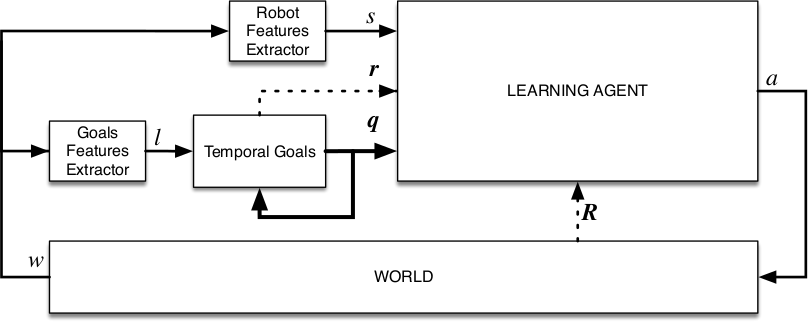
\includegraphics[width=0.75\textwidth]{images/rl-two-representations-no-borders}
	\end{figure}
	
	%		Notice: we have to deal with a joint transition model:
	%		\[Tr' = S \times \L \times A \to Prob(S, \L) \]
	
\end{frame}

\begin{frame}
	Our approach:
	\begin{itemize}
		\item Transform each $\varphi_i$ into \DFA $\automaton_{\varphi_i}$
		\item Do RL over an MDP $\MDP'$ with a transformed state space:
		\[S'= 
		\tikz[baseline]{
			\node[fill=yellow!20,anchor=base] (ts)
			{$S$};
		}
		\times 
		\tikz[baseline]{
			\node[fill=blue!20,anchor=base] (tq)
			{$Q_1 \times \dots \times Q_m$};
		}
		\]
	\end{itemize}
	
	%	\begin{tikzpicture}
	%	\end{tikzpicture}
	
	\begin{tikzpicture}
	\node[anchor=south west,inner sep=0] at (0,0) {		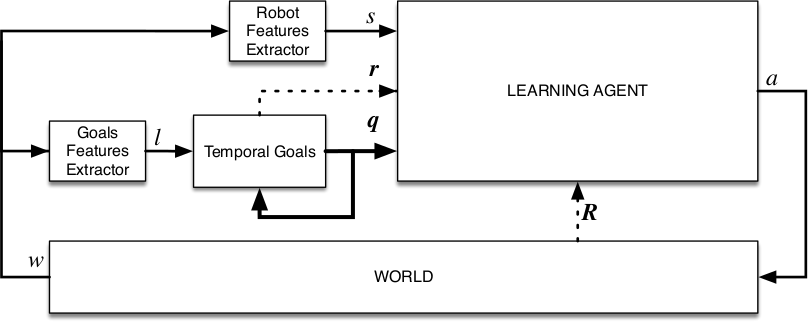
\includegraphics[width=0.9\textwidth]{images/rl-two-representations-no-borders}};
	%	\draw[red,ultra thick,rounded corners] (7.5,5.3) rectangle (9.4,6.2);
	%	\node [draw=red, anchor=base] (sl) at (1.95,2.25) {};
	\node [anchor=base] (sl) at (1.95,2.3) {};
	\node [anchor=base] (ss) at (4.65, 3.8) {};
	\node [anchor=base] (sq) at (4.65, 2.5) {};
	\end{tikzpicture}
	
	%	\begin{figure}
	%		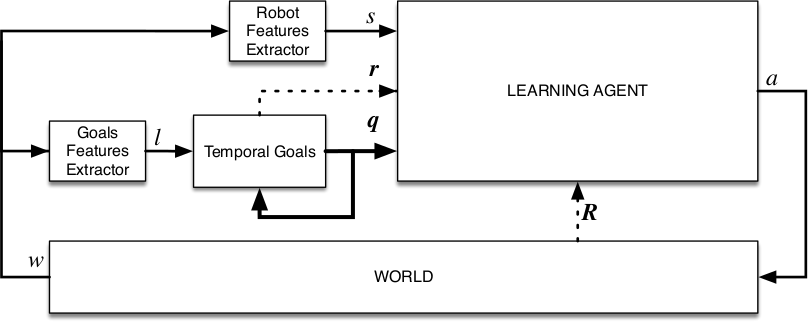
\includegraphics[width=0.9\textwidth]{images/rl-two-representations-no-borders}
	%	\end{figure}
	Notice: \textbf{the agent ignores the fluents} \tikz[baseline]{\node[fill=red!20,anchor=base] (tl) {$\L$}}!\\
	
	
	The actual RL relies on standard RL algorithms (e.g. Sarsa($\lambda$))
	
	% Now it's time to draw some edges between the global nodes. Note that we
	% have to apply the 'overlay' style.
	\begin{tikzpicture}[overlay]
	\path[->]<1-> (ts) edge [bend left] (ss);
	\path[->]<1-> (tq) edge [bend left] (sq);
	\path[->]<1-> (tl) edge [bend right] (sl);
	\end{tikzpicture}
	
\end{frame}


\begin{frame}{An optimal policy for \Sapientino}
	
	\LTLf goal $\varphi = \Diamond (red \land \Diamond (green \land \Diamond(blue)))$\\
	The equivalent \DFA is (roughly):
	
	\begin{center}
		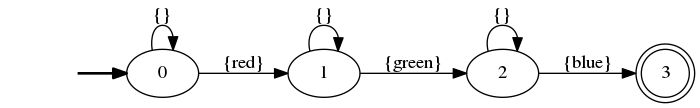
\includegraphics[width=\textwidth]{images//sapientino-simple-dfa-horizontal}
	\end{center}
	

\end{frame}


\begin{frame}{An optimal policy for \Sapientino}
		\LTLf goal $\varphi = \Diamond (red \land \Diamond (green \land \Diamond(blue)))$, reward $r = 300$\\
		
		\only<01>{Current state $s' = (x_4, y_3, 0)$, Action $a = start$}
		\only<02>{Current state $s' = (x_4, y_2, 0)$, Action $a = UP$}
		\only<03>{Current state $s' = (x_5, y_2, 0)$, Action $a = RIGHT$}
		\only<04>{Current state $s' = (x_6, y_2, 0)$, Action $a = RIGHT$}
		\only<05>{Current state $s' = (x_7, y_2, 0)$, Action $a = RIGHT$}
		\only<06>{Current state $s' = (x_7, y_2, 1)$, Action $a = BIP$, reward = +100}
		\only<07>{Current state $s' = (x_6, y_2, 1)$, Action $a = LEFT$}
		\only<08>{Current state $s' = (x_6, y_3, 1)$, Action $a = DOWN$}
		\only<09>{Current state $s' = (x_6, y_3, 2)$, Action $a = BIP$, reward = +100}
		\only<10>{Current state $s' = (x_6, y_4, 2)$, Action $a = DOWN$}
		\only<11>{Current state $s' = (x_7, y_4, 2)$, Action $a = RIGHT$}
		\only<12>{Current state $s' = (x_7, y_5, 2)$, Action $a = DOWN$}
		\only<13>{Current state $s' = (x_7, y_5, 3)$, Action $a = BIP$, reward $= +100$}
	\begin{table}

		\begin{tabular}{c c}
			
			%\includegraphics[width=0.5\textwidth]{images//sapientino-start} &	
			\includegraphics[width=0.6\textwidth]<01>{images//gifs/optimal-policy-three-colors/frame_00}
			\includegraphics[width=0.6\textwidth]<02>{images//gifs/optimal-policy-three-colors/frame_01}
			\includegraphics[width=0.6\textwidth]<03>{images//gifs/optimal-policy-three-colors/frame_02}
			\includegraphics[width=0.6\textwidth]<04>{images//gifs/optimal-policy-three-colors/frame_03}
			\includegraphics[width=0.6\textwidth]<05>{images//gifs/optimal-policy-three-colors/frame_04}
			\includegraphics[width=0.6\textwidth]<06>{images//gifs/optimal-policy-three-colors/frame_05}
			\includegraphics[width=0.6\textwidth]<07>{images//gifs/optimal-policy-three-colors/frame_06}
			\includegraphics[width=0.6\textwidth]<08>{images//gifs/optimal-policy-three-colors/frame_07}
			\includegraphics[width=0.6\textwidth]<09>{images//gifs/optimal-policy-three-colors/frame_08}
			\includegraphics[width=0.6\textwidth]<10>{images//gifs/optimal-policy-three-colors/frame_09}
			\includegraphics[width=0.6\textwidth]<11>{images//gifs/optimal-policy-three-colors/frame_10}
			\includegraphics[width=0.6\textwidth]<12,13>{images//gifs/optimal-policy-three-colors/frame_11}
			
			&
			
			\includegraphics[height=0.7\textheight]<01-05>{images//gifs/sapientino-simple-dfa/sapientino-simple-dfa-0}
			\includegraphics[height=0.7\textheight]<06-08>{images//gifs/sapientino-simple-dfa/sapientino-simple-dfa-1}
			\includegraphics[height=0.7\textheight]<09-12>{images//gifs/sapientino-simple-dfa/sapientino-simple-dfa-2}
			\includegraphics[height=0.7\textheight]<13>{images//gifs/sapientino-simple-dfa/sapientino-simple-dfa-3}
			\end{tabular}
	\end{table}
	
	
\end{frame}
\begin{frame}{Discussion about \Sapientino example}
	
	\textbf{Crucial remark}: the agent doesn't know \textbf{anything} about fluents!
	\begin{itemize}
		\item Great! \emph{Separation of concern} and \emph{modularity}
		\item He is aware that ``something changes" (automata transitions)
		\item Thanks to \emph{reward shaping}, he knows if it is a \emph{good/bad} transition
	\end{itemize}
	
	\vspace{0.5cm}
	\textbf{High expressive power}:
	\begin{itemize}
	\item Many different goals and constraints, e.g. exactly two visit per color in a given order, no bad visits in the meanwhile...
	
	\item We can use also \LDLf, expressive as \MSO (i.e. regular expressions)
	\end{itemize}
	
\end{frame}

\begin{frame}{About the two-fold representation}
	\textbf{Notice}: it seems that the agent \textbf{implicitly} learns where are the \emph{colors}, by knowing the \emph{coordinates}.\\
	
	\vspace{0.3cm}
	In \Sapientino, the agent can learn where are colors because each color can be associated to different coordinates.
	
	\vspace{0.3cm}
	In general, however, the correlation between $\L$ and $\S$ does not need to be formalized.
	\begin{itemize}
		\item $\L$ is the set of \textbf{high-level features}
		\item $\S$ is the set of \textbf{low-level features}
	\end{itemize}
	
	
\end{frame}

\begin{frame}{About the two-fold representation}
		
	\begin{block}{Question 1}
		Is a $\S$ minimal (and ``expressive enough'') wrt a $\L$?
	\end{block}
	
	\begin{block}{Question 2}
		What is the relationship b/w $\S$ and $\L$ to be satisfied, in order to allow the agent to accomplish the high-level tasks?
	\end{block}

	Answer: our approach makes no assumption about how the world works, hence we cannot give a general answer to these questions.\\
	
	\begin{itemize}
		\item The relationship b/w $\S$ and $\L$ is \textbf{highly environment-dependent}. One should restrict the set of worlds of interest and try to make some assumption.
		
		\item The ideal solution would be to have a constructive method that, given $\L$, allow us to build a proper $\S$.
	\end{itemize}

\end{frame}
\begin{frame}{About the two-fold representation}
	
	
	\textbf{Na\"ive solution}: put in $\S$ as many features as the designer consider useful, and run some feature selection techniques to cope with the complexity (e.g. by using Deep Learning)
	
	Famous examples:
	\begin{itemize}
		\item Mnih et al. 2015. \emph{Human-level control through deep reinforcement learning}. Nature 518(7540):529–533.
		\item Silver et al. 2017. \emph{Mastering the game of go without human knowledge}. Nature 550:354–359
	\end{itemize}
\end{frame}

\begin{frame}{\emph{Restraining Bolts}: AI safety}
	\url{https://www.starwars.com/databank/restraining-bolt}
	\begin{center}
	
\includegraphics[width=\textwidth]{images//restraining-bolt}
	\end{center}

\end{frame}

\begin{frame}{\emph{Restraining Bolts}: AI safety}
	
	Two distinct representations of the world:
	\begin{itemize}
		\item one by the agent, used for interacting with the world
		\item one by the \textbf{authority} imposing the bolt.
	\end{itemize}
	
	\vspace{0.3cm}
	With our approach, the agent must conform the restraining rules even if these are not expressed in its original	representation.\\
	
	\vspace{0.3cm}
	The agent can learn to act while conforming (as much as possible) to the \LLf specifications.\\
	
	
	
\end{frame}

\begin{frame}{\emph{Restraining Bolts}: AI safety}
	
	Our work would be to apply this concept to many different applications and scenarios.\\
	
	\vspace{0.3cm}
	The concept of safety guarantees is a hot topic and is of crucial importance in AI.
	\begin{itemize}
		\item Hadfield-Menell, Dylan, et al. \emph{The off-switch game.} arXiv preprint arXiv:1611.08219 (2016).
		\item Amodei, Dario, et al. \emph{Concrete problems in AI safety.} arXiv preprint arXiv:1606.06565 (2016).
	\end{itemize}
\end{frame}

\begin{frame}{Ad-hoc RL algorithms}
	One of the advantages of our method is to rely on standard RL algorithms.\\
	
	\vspace{0.5cm}
	However, it might be the case that ad-hoc algorithms leveraging the structure of our solution yield better performances.
\end{frame}

\begin{frame}{Ad-hoc RL algorithms: Options}
	
	\begin{itemize}
	\item Sutton et al., 1999. \emph{Between MDPs and semi-MDPs: A framework for temporal abstraction in reinforcement learning.} Artificial intelligence, 112(1-2), 181-211
	\end{itemize}
	
	\begin{center}
	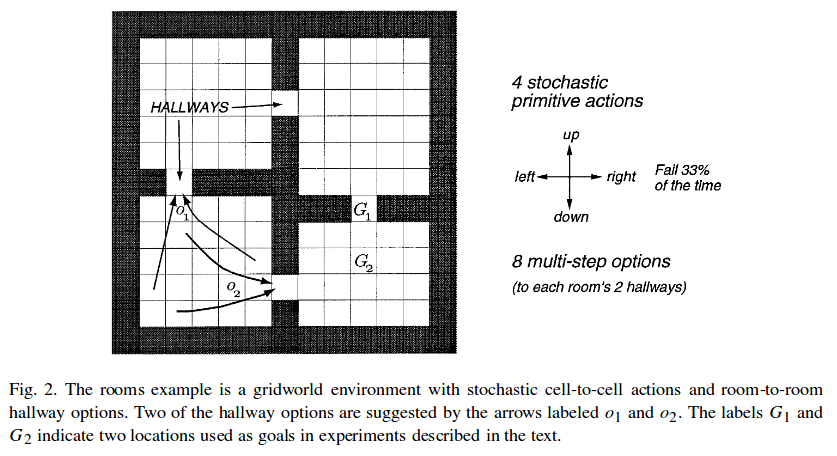
\includegraphics[width=0.8\linewidth]{images/options-paper-image}
	\end{center}
	
\end{frame}

\begin{frame}{Ad-hoc RL algorithms: Options}
	
	In our framework, \textbf{options might be associated with automata transition(s), or even the entire automata}.
	
	E.g. in the previous example with \Sapientino:
	\begin{itemize}
		\item reach any $red$ cell:
	\end{itemize}
	\begin{table}
		
		\begin{tabular}{c c}
			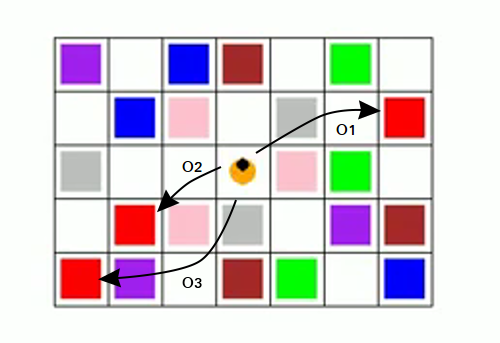
\includegraphics[width=0.6\textwidth]{images/sapientino-option-red}
			&
			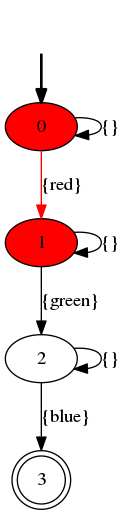
\includegraphics[height=0.6\textheight]{images/sapientino-simple-dfa-red-arrow}
		\end{tabular}
		
	\end{table}
	
\end{frame}

\begin{frame}{Ad-hoc RL algorithms: Options}
	Problem: we shouldn't specify by hand the needed options:
	\begin{itemize}
		\item it's not scalable
		\item it depends on choices about $\S$ and $\L$
	\end{itemize}
	
	\vspace{0.3cm}
	...But we can leverage the automaton (and reward shaping) to help the agent to learn options.
	
	Further considerations should be made to assess the applicability
	
	\vspace{0.3cm}
	Similar work:
	\begin{itemize}
		\item Stolle and Precup. 2002. \emph{Learning options in reinforcement learning.} International Symposium on abstraction, reformulation, and approximation. Springer, Berlin, Heidelberg.
	\end{itemize}
	
\end{frame}

\begin{frame}{Ad-hoc RL algorithms: Improve Exploration}
	\begin{itemize}
		\item Improve exploration (e.g. O-MCTS. M. de Waard et al., 2016).\\ In other words, focus on the next good \DFA state.
			
			\begin{center}
			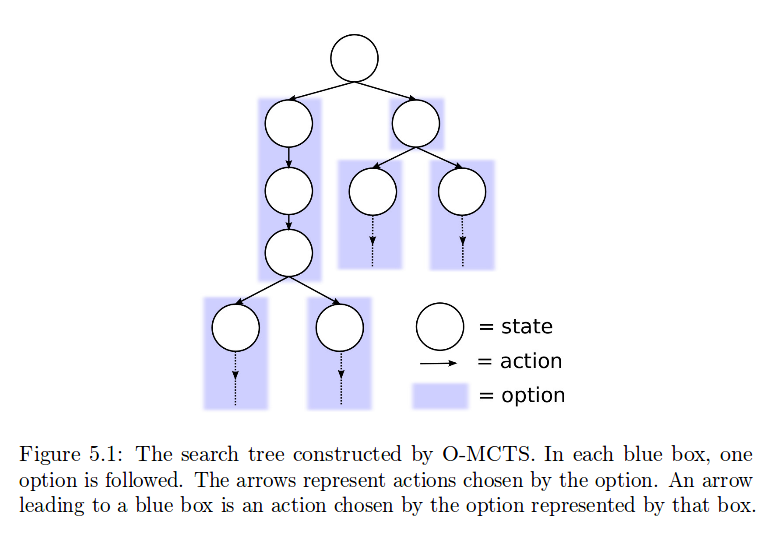
\includegraphics[width=0.7\textwidth]{images/o-mcts}
			\end{center}
			
	\end{itemize}
\end{frame}

\begin{frame}{Ad-hoc RL algorithms: Transfer Learning}
	\begin{itemize}
		\item Transfer learning: We can leverage past knowledge to accomplish other tasks.
	\end{itemize}
	E.g. \Sapientino:\\
	Consider a learned optimal policy $\pi$ for the goal $\tup{red, green, blue}$.\\
	We can leverage $\pi$ also for $\tup{pink, red, green, blue, brown}$ (and similar)
	
	\begin{center}
	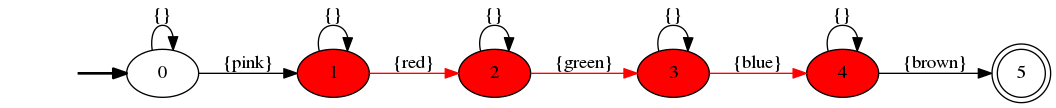
\includegraphics[width=\textwidth]{images/sapientino-composite-dfa-horizontal}
	\end{center}
	
	Assumption: $\pi$ is applicable after $0 \rightarrow 1$...
\end{frame}

\begin{frame}{Ad-hoc RL algorithms: other ideas}

	\begin{itemize}
		\item \textbf{Curriculum Learning}: focus the learning on a small part of a single automaton rather than every automaton in its entirety
		\item \textbf{Manifold representations}: Why only two representations? Generalize the approach to arbitrarily nested (high) representations:
		
		\begin{table}
			\begin{tabular}{c | c | c}
				& \textbf{set water temp} 	& add hot\\
				wake up		 		      & get wet 				    & add cold\\
				\textbf{have a shower}	  & shampoo 				    & ...\\
				have a breakfast	  	  & soap 					    & \\
				...						  & turn off water 			    & \\
				...						  & dry off 				    & 
			\end{tabular}
		\end{table}
		
		\item \textbf{Multi-agent systems}: extend the approach to multi-agent systems (e.g. automaton for common goal, shared high-level representation)
	\end{itemize}
		
\end{frame}

\begin{frame}{Reward Shaping improvements}
	Our system employs the use of (potential-based) reward shaping to facilitate the exploration, i.e.:
	
	Rewards are computed by simply split total rewards proportionally.
	
	\begin{center}
		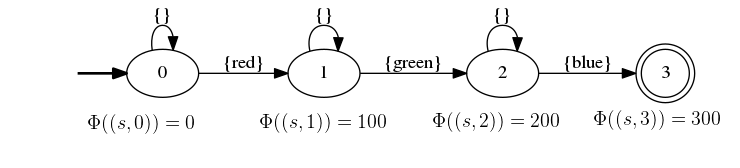
\includegraphics[width=\textwidth]{images/sapientino-simple-dfa-horizontal-with-potentials}
	\end{center}
	
	Reward shaping reduces to find a \emph{potential function} $\Phi(s):\S \to \mathbb{R}$. Guarantee of policy invariance (Ng et al., 1999)
\end{frame}

\begin{frame}{Reward Shaping improvements}
	Drawbacks of ``static" RS:
	\begin{itemize}
		\item \textbf{Fixed rewards}: potentials do not change according to the environment changes
		\item \textbf{Arbitrary rewards}: shaping rewards do not reflect the true ``hardness" an automaton transitions
	\end{itemize}
	
	Solutions:
	\begin{itemize}
		\item Employ \textbf{different rewards assignment schemes} (e.g. inverse proportion, attenuation factors)
		\item ``Shaping shaping rewards": update shaping rewards \emph{dynamically}, during the learning process, \textbf{proportionally to the \emph{hardness}} of the transitions (we should define \emph{hardness}...)
	\end{itemize}
\end{frame}
	
\begin{frame}{Miscellaneous}
	\begin{itemize}
		\item Extend the approach to different logical formalisms that can be translated to \DFA (e.g. \PLTL, \LTL safe, \LTL co-safe, ...)
		\item Improve existing implementations (i.e. RLTG\footnote{\url{https://github.com/MarcoFavorito/RLTG}}/ FLLOAT\footnote{\url{https://github.com/MarcoFavorito/FLLOAT}})
		\item Benchmarking with other approach on common task/environments
		\item Test the approach in many environments/contexts/goals (also physical ones)
	\end{itemize}

\end{frame}

\begin{frame}{Summary}
		Improvements and extensions of ``\emph{RL for \LLf goals}".
		
		\vspace{0.5cm}
		
		Experiments, experiments, experiments.
		
		\vspace{0.5cm}
		
		More generally, working in the middle of logic-based (i.e. Planning and Reasoning) and learning-based (i.e. Reinforcement Learning) approaches.
	
\end{frame}

\begin{frame}
	\begin{center}
	Thank you for your attention!
	\end{center}
\end{frame}

\end{document}
